
\chapter{Semiconductors}

\section{Intro}
Intro stuff goes here.

\section{Semiconductors}

\begin{figure}[htbp]
\begin{center}
\begin{tikzpicture}
%\draw[step=1cm,gray,very thin] (0,0) grid (12,5);
\draw (1,1) circle (0.5cm) node{A};
\draw (11,1) circle (0.5cm) node{B};
\draw (5.5,1) circle (0.5cm) node{A};
\draw (6.5,1) circle (0.5cm) node{B};
\draw (0,3) -- ++(2,0);
\draw (10,3) -- ++(2,0);
\draw (5,2) -- ++(2,0);
\draw (5,4) -- ++(2,0);
\draw[dashed] (2,3) -- (5,2);
\draw[dashed] (2,3) -- (5,4);
\draw[dashed] (10,3) -- (7,2);
\draw[dashed] (10,3) -- (7,4);
\draw[thick,->] (0.5,3) -- ++(0,0.5);
\draw[thick,<-] (10.5,3) -- ++(0,0.5);
\draw[thick,->] (5.5,2) -- ++(0,0.5);
\draw[thick,<-] (6.5,2) -- ++(0,0.5);
%\node at (1,1) {A};
\end{tikzpicture}
\caption{When two identical atoms A and B are brought close together, the two degenerate energy eigenstates for an electron (located at atom A or B) are replaced with two states of differing energy, equally shared between atoms A and B.}
\label{fig:bond}
\end{center}
\end{figure}

Consider the simple quantum mechanical model illustrated in Fig.~\ref{fig:bond}.  When two identical atoms, A and B, are very far apart, they can be considered separately, and the energy eigenstates are degenerate in energy.  For each solution for an electron located at atom A, there is a solution of equal energy for an electron located at atom B.  When the atoms A and B are brought close enough together, a particle located at atom A can quantum mechanically tunnel to atom B, and so these states are no longer energy eigenstates.  Instead, the eigenstates share the electron equally between A and B, in either a symmetric or antisymmetric wave function.  The symmetric wave function has lower energy than the antisymmetric wave function, so that the energy levels are no longer degenerate.  If the outer most level is not full, this results in a lower total energy through sharing, which is the quantum mechanical explanation for a covalent bond.

\begin{figure}[htbp]
\begin{center}
\begin{tikzpicture}
\draw (0,3) -- ++(1,0);
\draw (2,4) -- ++(1,0);
\draw (2,2) -- ++(1,0);
\draw (4,4.5) -- ++(1,0);
\draw (4,3.5) -- ++(1,0);
\draw (4,2.5) -- ++(1,0);
\draw (4,1.5) -- ++(1,0);
\draw (6,1.0) -- ++(1,0);
\draw (6,1.5) -- ++(1,0);
\draw (6,2.0) -- ++(1,0);
\draw (6,2.5) -- ++(1,0);
\draw (6,3.0) -- ++(1,0);
\draw (6,3.5) -- ++(1,0);
\draw (6,4.0) -- ++(1,0);
\draw (6,4.5) -- ++(1,0);
\draw (6,5.0) -- ++(1,0);
\node at (0.5,0.5) {$n=1$};
\node at (2.5,0.5) {$2$};
\node at (4.5,0.5) {$4$};
\node at (6.5,0.5) {$8$};
\node at (8.5,0.5) {$10^{23}$};
\draw[thick] (8,0.75) rectangle (9,5.25);
\end{tikzpicture}
\caption{As more and more identical atoms are brought close together, the number of distinct energy levels increases until there is an effectively continuous band of available energies.}
\label{fig:bands}
\end{center}
\end{figure}

\begin{figure}[htbp]
\begin{center}
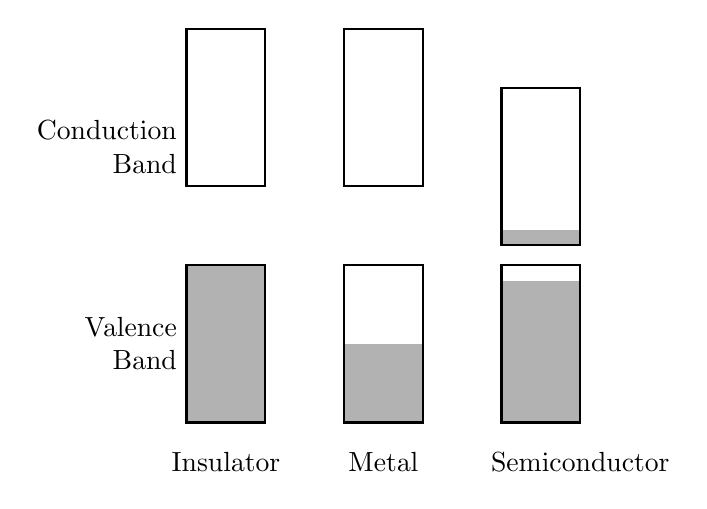
\begin{tikzpicture}
%\draw[step=1cm,gray,very thin] (0,0) grid (6,6);
\fill[black!30!white] (0,1) rectangle ++(1,2);
\draw[thick] (0,1) rectangle ++(1,2);
\draw[thick] (0,4) rectangle ++(1,2);
\fill[black!30!white] (2,1) rectangle ++(1,1);
\draw[thick] (2,1) rectangle ++(1,2);
\draw[thick] (2,4) rectangle ++(1,2);
\fill[black!30!white] (4,1) rectangle ++(1,1.8);
\fill[black!30!white] (4,3.25) rectangle ++(1,0.2);
\draw[thick] (4,1) rectangle ++(1,2);
\draw[thick] (4,3.25) rectangle ++(1,2);
\node[left, align=right] at (0,4.5) {Conduction \\ Band};
\node[left, align=right] at (0,2) {Valence \\Band};
\node at (0.5,0.5) {Insulator};
\node at (2.5,0.5) {Metal};
\node at (5.0,0.5) {Semiconductor};
\end{tikzpicture}
\caption{The valance and conduction bands for insulators, metals, and semiconductor.  The shared regions indicate electrons}
\label{fig:materials}
\end{center}
\end{figure}

Now consider what happens when an Avagadro's number ($\sim 10^{23}$) of molecules or atoms are brought together to form a periodic lattice.  As illustrated in Fig.~\ref{fig:bands} each discrete energy level in the single atom is replaced by a nearly continuous band of available energies in the lattice.  Many of the important properties of materials can be understood by considering only the energy band that contains the highest energy electron (called the valance band) and the band directly above it (called the conduction band).  

As shown in Fig.~\ref{fig:materials}, an insulator consists of a full valence band separated from the conduction band by a large gap.  The complete set of possible wave functions for an electron in the valance band can be though of as left-traveling and right-traveling waves.  From symmetry there are an equal number of left and right traveling waves.  When a band is full, there are therefore always an equal number of left and right traveling waves and no net current.  A metal has a partially full valance band, and therefore no difficulty conducting charge.

A semiconductor contains a full valance band separated from the conductor by a small band gap.  As a result, thermal fluctuations allow electrons in the valance band to gain sufficient energy to enter the conduction band, leaving an unfilled state in the valance band.  The electrons in the conduction band can conduct electricity.  The vacant states in the valance band can also conduct electricity, as the absence of a negative charge acts like a mobile positive charge, which is called a hole.

Intrinsic semiconductors have an equal number of electrons and holes.  However, in a process called doping, different molecules are added periodically to the semiconductor lattice that tend to provide additional electrons to the conduction band or absorb additional electrons from the valance band.  This leads to either an excess of holes in $p$-type semiconductors and an excess in electrons in $n$-type semiconductors.  Semiconductors are the core technology upon which the entire modern electronics industry is based.

\section{The Diode}

\begin{figure}[htbp]
\begin{center}
\begin{tabular}{cc}
\begin{circuitikz}[line width=1pt]
%\draw (0,0) to[voltage source,bipoles/length=1.5cm,l=$V$] ++(0,+3.0) to[D] ++(3.0,0);
\draw(0,0) to[D] ++(3,0);
\end{circuitikz} &
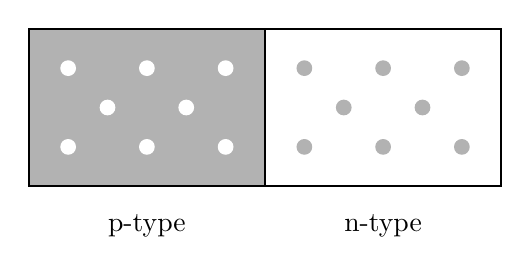
\begin{tikzpicture}
%\draw[step=1cm,gray,very thin] (0,0) grid (6,3);
\fill[black!30!white] (0,1) rectangle ++(3,2);
\draw[thick] (0,1) rectangle ++(3,2);
\draw[thick] (3,1) rectangle ++(3,2);
\fill[white] (0.5,1.5) circle (0.10);
\fill[white] (0.5,2.5) circle (0.10);
\fill[white] (1.5,1.5) circle (0.10);
\fill[white] (1.5,2.5) circle (0.10);
\fill[white] (2.5,1.5) circle (0.10);
\fill[white] (2.5,2.5) circle (0.10);
\fill[white] (1,2) circle (0.10);
\fill[white] (2,2) circle (0.10);
\fill[black!30!white] (3.5,1.5) circle (0.10);
\fill[black!30!white] (3.5,2.5) circle (0.10);
\fill[black!30!white] (4.5,1.5) circle (0.10);
\fill[black!30!white] (4.5,2.5) circle (0.10);
\fill[black!30!white] (5.5,1.5) circle (0.10);
\fill[black!30!white] (5.5,2.5) circle (0.10);
\fill[black!30!white] (4,2) circle (0.10);
\fill[black!30!white] (5,2) circle (0.10);
\node at (1.5,0.5) {p-type};
\node at (4.5,0.5) {n-type};
\end{tikzpicture}
\\
(a)&
(b)\\
\end{tabular}
\caption{The diode (a) circuit diagram, and (b) as a junction between p-type and n-type semiconductor.  The white circles represent holes and the gray circles represent electrons.}
\label{fig:diode}
\end{center}
\end{figure}

\begin{figure}[htbp]
\begin{center}
\begin{tabular}{cc}
\begin{circuitikz}[line width=1pt]
\draw (0,0) to[short,i<=$I$] ++(0,+3.0) to[D] ++(3.0,0);
\draw (0,0) to[short] ++(3,0) to[voltage source,bipoles/length=1.5cm] ++(0,3);
\end{circuitikz} &
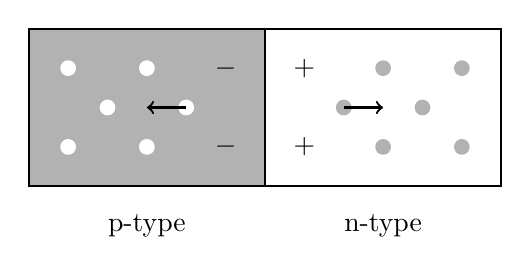
\begin{tikzpicture}
%\draw[step=1cm,gray,very thin] (0,0) grid (6,3);
\fill[black!30!white] (0,1) rectangle ++(3,2);
\draw[thick] (0,1) rectangle ++(3,2);
\draw[thick] (3,1) rectangle ++(3,2);
\fill[white] (0.5,1.5) circle (0.10);
\fill[white] (0.5,2.5) circle (0.10);
\fill[white] (1.5,1.5) circle (0.10);
\fill[white] (1.5,2.5) circle (0.10);
%\fill[white] (2.5,1.5) circle (0.10);
%\fill[white] (2.5,2.5) circle (0.10);
\node at (2.5,1.5) {$-$};
\node at (2.5,2.5) {$-$};
\fill[white] (1,2) circle (0.10);
\fill[white] (2,2) circle (0.10);
%\fill[black!30!white] (3.5,1.5) circle (0.10);
%\fill[black!30!white] (3.5,2.5) circle (0.10);
\node at (3.5,1.5) {$+$};
\node at (3.5,2.5) {$+$};
\fill[black!30!white] (4.5,1.5) circle (0.10);
\fill[black!30!white] (4.5,2.5) circle (0.10);
\fill[black!30!white] (5.5,1.5) circle (0.10);
\fill[black!30!white] (5.5,2.5) circle (0.10);
\fill[black!30!white] (4,2) circle (0.10);
\fill[black!30!white] (5,2) circle (0.10);
\draw[thick,->] (4,2) -- ++(0.5,0);
\draw[thick,->] (2,2) -- ++(-0.5,0);
\node at (1.5,0.5) {p-type};
\node at (4.5,0.5) {n-type};
\end{tikzpicture}
\\
(a)&
(b)\\
\end{tabular}
\caption{The diode is in reverse bias when the (a) the applied voltage directs a positive current through the diode opposite the arrow in the diode diagram, and (b) which tends to pull mobile holes and electrons away from the p-n junction, creating a depletion zone.}
\label{fig:dioderev}
\end{center}
\end{figure}


\begin{figure}[htbp]
\begin{center}
\begin{tabular}{cc}
\begin{circuitikz}[line width=1pt]
\draw (0,0) to[voltage source,bipoles/length=1.5cm,i>=$I$] ++(0,+3.0) to[D] ++(3.0,0) |- (0,0);
\end{circuitikz} &
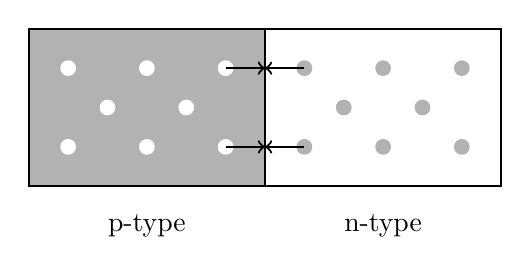
\begin{tikzpicture}
%\draw[step=1cm,gray,very thin] (0,0) grid (6,3);
\fill[black!30!white] (0,1) rectangle ++(3,2);
\draw[thick] (0,1) rectangle ++(3,2);
\draw[thick] (3,1) rectangle ++(3,2);
\fill[white] (0.5,1.5) circle (0.10);
\fill[white] (0.5,2.5) circle (0.10);
\fill[white] (1.5,1.5) circle (0.10);
\fill[white] (1.5,2.5) circle (0.10);
\fill[white] (2.5,1.5) circle (0.10);
\fill[white] (2.5,2.5) circle (0.10);
\fill[white] (1,2) circle (0.10);
\fill[white] (2,2) circle (0.10);
\fill[black!30!white] (3.5,1.5) circle (0.10);
\fill[black!30!white] (3.5,2.5) circle (0.10);
\fill[black!30!white] (4.5,1.5) circle (0.10);
\fill[black!30!white] (4.5,2.5) circle (0.10);
\fill[black!30!white] (5.5,1.5) circle (0.10);
\fill[black!30!white] (5.5,2.5) circle (0.10);
\fill[black!30!white] (4,2) circle (0.10);
\fill[black!30!white] (5,2) circle (0.10);
\node at (1.5,0.5) {p-type};
\node at (4.5,0.5) {n-type};
\draw[thick,->] (2.5,1.5) -- (3.0,1.5);
\draw[thick,->] (2.5,2.5) -- (3.0,2.5);
\draw[thick,->] (3.5,1.5) -- (3.0,1.5);
\draw[thick,->] (3.5,2.5) -- (3.0,2.5);
\end{tikzpicture}
\\
(a)&
(b)\\
\end{tabular}
\caption{The diode is in forward bias when the (a) applied voltage directs a positive current in the same direction as the arrow in the diode symbol, and (b) tends to move electrons and holes toward the pn junction, where they recombine. }
\label{fig:diodefwd}
\end{center}
\end{figure}

A diode is a junction of $p$-type and $n$-type semiconductor as shown in Fig.~\ref{fig:diode}.   The diode has an interesting and useful $V$-$I$ curve that depends on the polarity of the applied voltage.  Consider first what happens if we apply a reverse-bias voltage as illustrated in Fig.~\ref{fig:dioderev}.  In this configuration, the applied voltage initially creates a current which move holes to left and electrons to right, which in both cases moves the mobile charge carriers away from the pn junction.  This creates a depletion zone at the junction with no mobile charge carriers.  Because the semiconductors initially had no net charge, as holes move out of the depletion zone in the p-type semiconductor, they leave behind a fixed negative charge.  Likewise, as electrons move out of the depletion zone in the n-type semiconductor, the leave behind a fixed positive charge.  The fixed charges create an electric field which results in a voltage across the depletion zone.  The depletion zone widens until the voltage across the depletion zone equals the applied voltage, at which point no current flows.  In the steady-state, a diode in reverse bias passes no current.  

Now consider what happens if we apply a forward-bias voltage as illustrated in Fig.~\ref{fig:dioderev}.  In this configuration, the applied voltage produces a current which moves holes to right and electrons to the left, which in both cases moves the mobile charge carriers toward the pn junction.  At this junction, the electrons recombine with holes, which allows a current in this direction to continue as long as the voltage is applied.


\begin{figure}[htbp]
\begin{center}
\begin{tabular}{p{2cm}p{2cm}p{2cm}c}
\begin{circuitikz}[line width=1pt]
\draw(0,0) to[D] ++(0,-3);
\end{circuitikz} &
\begin{circuitikz}[line width=1pt]
\draw(0,0) to[short,-o] ++(0,1);
\draw(0,2) to[short,o-] ++(0,1);
\end{circuitikz} &
\begin{circuitikz}[line width=1pt]
\draw(0,0) to[voltage source,bipoles/length=1.5cm,l=$V_{\rm d}$] ++(0,3);
\end{circuitikz} &
\includegraphics[width=0.45\textwidth]{figs/diodeop.pdf} \\
(a) & (b) & (c) & (d) \\
\end{tabular}
\caption{Circuit diagram from a (a) diode, equivalent circuits for (b) reverse bias and (c) forward bias, and   the corresponding (d) IV curve.  For a typical silicon diode $V_{\rm D}$ is between $0.6$ and $0.7~\rm V$.}
\label{fig:diodeeqv}
\end{center}
\end{figure}

A diode, therefore, has the very useful feature that it only allows current to flow in one direction.  As shown in Fig.~\ref{fig:diodeeqv} under reverse-bias the diode is equivalent to an open circuit.  Our discussion so far might lead you to think that under forward-bias, the diode is equivalent to a short circuit.  The situation is in fact slightly more complicated.  Absent any applied voltage, thermal fluctuations cause electrons and holes to bump into each other and combine at the pn junction, which causes a small depletion zone to form.   Meanwhile, thermal fluctuations also cause electrons in the valence band to reach the conduction band, creating electron-hole pairs.  The depletion zone increases until an equilibrium is reached between recombination and pair production.  This intrinsic depletion zone is effectively an voltage drop that must be overcome before any current can flow.  The equivalent circuit for a diode in forward bias is therefore a small voltage drop $V_{\rm d}$ as shown in Fig.~\ref{fig:diodeeqv}.  For typical silicon diodes, $V_{\rm d}$ is $0.6$ to $0.7~\rm V$.  Note that the direction of the allowed current in the diode assures us that the diode always consumes power.  It is a passive component and cannot be used to add power to a circuit.

\section{Current Rectification}

\begin{figure}[htbp]
\begin{center}
\begin{tabular}{cc}
\begin{circuitikz}[line width=1pt]
\draw (0,0) node[ground,yscale=2.0]{} to[sinusoidal voltage source,bipoles/length=1.5cm] ++(0,+3.0) 
to[D] ++(3.0,0) coordinate(X) to[R,l=$R_{\rm L}$] ++(0,-3) to[short,-*] ++(-3,0);
\draw (X) to[short,*-o] ++(0.75,0) node[right]{$v_{\rm R}(t)$};
\draw (0.0,2.2) node[left]{$v_{\rm S}(t)$};
\end{circuitikz} &
\includegraphics[width=0.55\textwidth]{figs/rectification.pdf} 
\\
(a) & (b) \\
\end{tabular}
\caption{ Half-wave rectifier}
\label{fig:basicrect}
\end{center}
\end{figure}

In the previous section, we discussed that operationally, a diode is an open circuit under reverse bias, and  a constant voltage drop $V_D$ under forward bias.  The IV curve for this operational model of the diode shown in Fig.~\ref{fig:diodeeqv} is usually sufficient for understanding the behavior of circuits involving diodes.  The rectification feature of a diode is illustrated in Fig.~\ref{fig:basicrect}.  The voltage across the resistor is the positive half of the source AC voltage, reduced by one diode drop.

\begin{figure}[htbp]
\begin{center}
\begin{tabular}{cc}
\begin{circuitikz}[line width=1pt]
\draw (0,0) node[ground,yscale=2.0]{} to[sinusoidal voltage source,bipoles/length=1.5cm] ++(0,+3.0) 
to[D] ++(2.0,0) coordinate(X) to[C,l=$C$] ++(0,-3) to[short,-*] ++(-2,0);
\draw (X) to[short,*-] ++(1.0,0) coordinate(X) to[R,l=$R_{\rm L}$] ++(0,-3) to[short,-*] ++(-1,0);
\draw (X) to[short,*-o] ++(0.75,0) node[right]{$v_{\rm R}(t)$};
\draw (0.0,2.2) node[left]{$v_{\rm S}(t)$};
\end{circuitikz} &
\includegraphics[width=0.55\textwidth]{figs/ripple.pdf} 
\\
(a) & (b) \\
\end{tabular}
\caption{ Half-wave rectifier with capacitor.}
\label{fig:ripple}
\end{center}
\end{figure}

The voltage across the resistor $R_{\rm L}$ (and corresponding current) for the half-wave rectifier circuit in Fig.~\ref{fig:basicrect} has a non-zero DC component, but it varies significantly as a function of time.  To produce a more constant DC voltage, a capacitor can be used as in Fig.~\ref{fig:ripple}.  The capacitor provides current to the load during the portion of the cycle when the rectified AC voltage is too low.
As the capacitor provides current to the load, it's voltage sags, resulting in AC ripple current in addition to the DC voltage.  The ripple current can be reduced by increasing the size of the capacitor.  We can estimate the size of the ripple current by considering that the voltage sag $\Delta v$ is given by:
\begin{displaymath}
\Delta v = \frac{\Delta q}{C}.
\end{displaymath}
Meanwhile, the most the capacitor can discharge during the cycle of frequency $f=1/T$ is:
\begin{displaymath}
\Delta q = I_{\rm max} \, T = \frac{I_{\rm max}}{f}  
\end{displaymath}
And so the voltage sag is:
\begin{displaymath}
\Delta v = \frac{I_{\rm max}}{fC} = \frac{V_{\rm max}}{fRC}.
\end{displaymath}

\section{Real Diodes}

\begin{figure}[htbp]
\begin{center}
\begin{tabular}{cc}
\includegraphics[width=0.45\textwidth]{figs/diodeeq.pdf} &
\includegraphics[width=0.45\textwidth]{figs/breakdown.pdf} \\
(a) &
(b) \\
\end{tabular}
\caption{Diode $I$-$V$ curve (a) from the Schockley equations, and (b) from the Schockley equations at wider scale and including breakdown.  Typical values of $V_{\rm T} = 26~\rm mV$, $I_{\rm S} = 5~\rm \mu A$, $V_{\rm D}=0.6~\rm V$}
\label{fig:diodeeqs}
\end{center}
\end{figure}

The useful operational model of the diode differs from real diodes in several ways.  While under reverse bias, thermal fluctuations in the depletion band of diode produce a small but constant supply of mobile charge carriers, which allows a small current to flow under reverse bias.  This current, called the saturation current $I_{\rm S}$ is quite small.  For the 1N914 diode, $I_{\rm S} = 5~\rm \mu A$.
If the reverse bias voltage is increased sufficiently, the small number of mobile charge carriers forming the saturation current are accelerated enough to produce additional electron-hole pairs through collisions, creating a cascade that dramatically increases the reverse current.   Diodes typically have a breakdown voltage below which they will conduct in reverse-bias.  Instead of avalanche breakdown, some diodes breakdown due to quantum tunnelng, by an effect called Zener breakdown.  Zener diodes are specifically designed to provide a nearly constant voltage under reverse bias, and are often used to regulate DC voltage levels.

A full thermodynamic treatment of the pn junction in a diode yields the Schockley diode equation:
\begin{displaymath}
I(V) = I_{\rm S} \left( \exp\left( \frac{V}{V_{\rm T}}\right) - 1 \right)
\end{displaymath}
where $V_{\rm T}$ is the thermal voltage, defined by 
\begin{displaymath}
V_{\rm T} = \frac{kT}{e},
\end{displaymath}
which has the value $26~\rm mV$ at room temperature.  The diode equation is plotted in Fig.~\ref{fig:diodeeqs}a at a scale where the exponential behavior and reverse current are visible.  In Fig.~\ref{fig:diodeeqs}b the scale is adjusted to typical scale for circuit parameters, and the curve much more closely resembles the simple operational model. 

\appendix

\chapter{Practice Problems}

\section{DC Circuits}

\begin{enumerate}

\item In the circuit below, which includes a current source providing a constant $5~\rm mA$ current, find the indicated current $I$: \\
\begin{center}
\begin{circuitikz}[line width=1pt]
\draw (0,0) to[current source,bipoles/length=1.5cm] ++(0,+3.0) 
to[short] ++(1.5,0) coordinate(X) to[R,l=$2~\rm k\Omega$] ++(0,-3) to[short] ++(-1.5,0);
\draw (X) to[short,*-] ++(1.5,0) coordinate(X) to[R,l=$3~\rm k\Omega$,i=$I$] ++(0,-3) to[short,-*] ++(-1.5,0);
\draw (-0.25,2.0) node[left]{$5~\rm mA$};
\end{circuitikz} 
\end{center}

\item In the circuit below, find the voltage $V_{\rm out}$:
\begin{center}
\begin{circuitikz}[line width=1pt]
\draw (0,0) node[ground,yscale=2.0]{} to[voltage source,bipoles/length=1.5cm,l=$5~\rm V$] ++(0,+3.0) 
to[R,l=$2~\rm k\Omega$] ++(3.0,0) coordinate(X) to[R,l=$3~\rm k\Omega$] ++(0,-3) to[short] ++(-3.0,0);
\draw (X) to[short,*-o] ++(1.5,0) node[right]{$V_{\rm out}$};
\end{circuitikz} 
\end{center}


\item In the circuit below, find the indicated current $I$ in terms $V_{\rm out}$ and $R$:
\begin{center}
\begin{circuitikz}[line width=1pt]
\draw (0,0) to[voltage source,bipoles/length=1.5cm,l=$V_0$] ++(0,+3.0) 
to[R,l=$R$] ++(3.0,0) coordinate(X) to[R,l=$R$] ++(0,-3) to[short] ++(-3.0,0);
\draw (X) to[short] ++(1.5,0) to[R,l=$R$,i=$I$] ++(0,-3) to[short] ++(-3.0,0);
\end{circuitikz} 
\end{center}


\item In the circuit below, find the indicated current $I$ in terms of the DC voltage $V_{\rm out}$, and the component values $R$, and $C$:
\begin{center}
\begin{circuitikz}[line width=1pt]
\draw (0,0) to[voltage source,bipoles/length=1.5cm,l=$V_0$] ++(0,+3.0) 
to[short,i=I] ++(3.0,0) coordinate(X) to[C,l=$C$] ++(0,-3) to[short] ++(-3.0,0);
\draw (X) to[short] ++(1.5,0) to[R,l=$R$] ++(0,-3) to[short] ++(-3.0,0);
\end{circuitikz} 
\end{center}

\item In the circuit below, find the indicated current $I$ in terms of the DC voltage $V_{\rm out}$, and the component values $R$, and $C$:
\begin{center}
\begin{circuitikz}[line width=1pt]
\draw (0,0) to[voltage source,bipoles/length=1.5cm,l=$V_0$] ++(0,+3.0) 
to[C,l=$C$] ++(3.0,0) to[R,l=$R$,i=$I$] ++(0,-3) to[short] ++(-3.0,0);
\end{circuitikz} 
\end{center}

\item In the circuit below, which includes an inductor with inductance $L$, find the indicated current $I$ in terms of the DC voltage $V_{\rm out}$, and the component values $L$, and $R$:
\begin{center}
\begin{circuitikz}[line width=1pt]
\draw (0,0) to[voltage source,bipoles/length=1.5cm,l=$V_0$] ++(0,+3.0) 
to[L,l=$L$] ++(3.0,0) to[R,l=$R$,i=$I$] ++(0,-3) to[short] ++(-3.0,0);
\end{circuitikz} 
\end{center}

\item Find the Thevenin equivalent circuit for the following two node network, expressing $V_{\rm th}$ and $R_{\rm th}$ in terms of the quantities $V_0$ and $R$:

\begin{center}
\begin{circuitikz}[line width=1pt]
\draw (0,0) coordinate(X) to[voltage source,bipoles/length=1.5cm,l=$V_0$] ++(0,+3.0) 
to[R,l=$R$,-o] ++(3.0,0) node[right]{B};
\draw (X) to[R,l=$R$,-o] ++(3.0,0) node[right]{A};
\end{circuitikz} 
\end{center}

\newpage

\item Find the Thevenin equivalent circuit for the following two node network, expressing $V_{\rm th}$ and $R_{\rm th}$ in terms of the quantities $V_0$ and $R$:

\begin{center}
\begin{circuitikz}[line width=1pt]
\draw (0,0) to[voltage source,bipoles/length=1.5cm,l=$V_0$] ++(0,+3.0) 
to[R,l=$R$] ++(3.0,0) coordinate(X) to[short,*-o] ++(1.0,0) node[right]{B};
\draw (X) to[R,l=$R$,-o] ++(0.0,-3.0) coordinate(X) to[short,*-o] ++(1.0,0) node[right]{A};
\draw(X) to[short,*-] ++(-3.0,0);
\end{circuitikz} 
\end{center}

\item Find the Thevenin equivalent circuit for the following two node network, expressing $V_{\rm th}$ and $R_{\rm th}$ in terms of the quantities $V_0$ and $R$:

\begin{center}
\begin{circuitikz}[line width=1pt]
\draw (0,0) to[voltage source,bipoles/length=1.5cm,l=$V_0$] ++(0,+3.0) 
to[short] ++(1.5,0) coordinate(X) to[short,*-o] ++(1.0,0) node[right]{B};
\draw (X) to[R,l=$R$,-o] ++(0.0,-3.0) coordinate(X) to[short,*-o] ++(1.0,0) node[right]{A};
\draw(X) to[short,*-] ++(-1.5,0);
\end{circuitikz} 
\end{center}

\item Find the Thevenin equivalent circuit for the following two node network,
expressing $V_{\rm th}$ and $R_{\rm th}$ in terms of the constant current $I_0$ and the resistance $R$:

\begin{center}
\begin{circuitikz}[line width=1pt]
\draw (0,0) to[current source,bipoles/length=1.5cm,l=$I_0$] ++(0,+3.0) 
to[short] ++(1.5,0) coordinate(X) to[short,*-o] ++(1.0,0) node[right]{B};
\draw (X) to[R,l=$R$,-o] ++(0.0,-3.0) coordinate(X) to[short,*-o] ++(1.0,0) node[right]{A};
\draw(X) to[short,*-] ++(-1.5,0);
\end{circuitikz} 
\end{center}

\item Find the Thevenin equivalent circuit for the following two node network,
expressing $V_{\rm th}$ and $R_{\rm th}$ in terms of the resistance $R$:

\begin{center}
\begin{circuitikz}[line width=1pt]
\draw (0,0) node[right]{A} to[short,o-] ++(-2.5,0) to[R,l=$R$,-*] ++(0.0,1.5) coordinate(X);
\draw (X) to[short] ++(-0.75,0) to[R,l=$R$] ++(0.0,1.5) to[short,-o] ++(3.25,0) node[right]{B};
\draw (X) to[short] ++(0.75,0) to[R,l=$R$,-*] ++(0.0,1.5);
\end{circuitikz} 
\end{center}



\item Find the Thevenin equivalent circuit for the following two node network, expressing $V_{\rm th}$ and $R_{\rm th}$ in terms of the quantities $V_0$ and $R$:

\begin{center}
\begin{circuitikz}[line width=1pt]
\draw (0,0) coordinate(X) to[R,l=$R$] ++(0,1.5) coordinate(Y) to[short] ++(0,1.5) to[R,l=$R$] ++(0,1.5);
\draw (Y) to[short,*-] ++(1.5,0) to[voltage source,bipoles/length=1.5cm,l=$V_0$] ++(0,1.5) to[short,-*] ++(1.5,0);
\draw (X) to[short] ++(3.0,0) coordinate(X);
\draw (X) to[R,l=$R$] ++(0,1.5) to[short] ++(0,1.5) to[R,l=$R$] ++(0,1.5) coordinate(Y);
\draw (Y) to[short] ++(-3.0,0);
\draw (X) to[short,-o] ++(1.0,0) node[right]{A};
\draw (Y) to[short,-o] ++(1.0,0) node[right]{B};
\end{circuitikz} 
\end{center}


\item Find the Thevenin equivalent circuit for the following two node network, expressing $V_{\rm th}$ and $R_{\rm th}$ in terms of the constant current $I_0$ and the resistance $R$:

\begin{center}
\begin{circuitikz}[line width=1pt]
\draw (0,0) to[R,l=$R$] ++(0,1.5) to[R,l=$R$] ++(0,1.5) to[short] ++(2.5,0) coordinate(X);
\draw (X) to[short,-o] ++(1.0,0) node[right]{B};
\draw (X) to[R,l_=$R$,*-] ++(0,-1.5) coordinate(X) to[current source,bipoles/length=1.5cm,l=$I_0$,-*] ++(-2.5,0);
\draw (X) to[R,l_=$R$,*-] ++(0,-1.5) coordinate(X) to[short] ++ (-2.5,0);
\draw (X) to[short,-o] ++(1.0,0) node[right]{A};
\end{circuitikz} 
\end{center}


\item Circuits like the one below, which contains the bridge resistor $R_3$, cannot be reduced in terms of series and parallel resistors.  For this particular circuit, we'll show that $I_1 = I_5$ and $I_2 = I_4$, which seems plausible based on symmetry.
\begin{center}
\begin{circuitikz}[line width=1pt]
\draw (0,0) to[R,l=$R_2$,i<^=$I_4$] ++(0,3.0) to[R,l=$R_1$,i<=$I_1$] ++(0,3.0) to[short] ++(3.0,0) coordinate(X);
\draw (X) to[R,l_=$R_2$,i>_=$I_2$] ++(0,-3.0) coordinate(X) to[R,l=$R_3$,i<^=$I_3$,-*] ++(-3.0,0);
\draw (X) to[R,l_=$R_1$,i_>=$I_5$,*-] ++(0,-3.0) coordinate(X) to[short] ++ (-3.0,0) coordinate(X);
\draw(X) to[short,*-] ++(-3.0,0) to[voltage source,bipoles/length=1.5cm,l=$V_0$] ++(0,6.0) 
to[short,i=$I$,*-] ++(3.0,0);
\end{circuitikz} 
\end{center}
First show why:
\begin{eqnarray*} 
I_1 + I_2 &=& I_4 + I_5 \\
I_1 R_1 + I_4 R_2 &=& I_2 R_2 + R_1 I_5 \\
\end{eqnarray*}
then use these equations to show that we must have:
\begin{eqnarray*} 
I_1 &=& I_5 \\
I_2 &=& I_4 \\
\end{eqnarray*}

\item Consider the bridge circuit below, which has been simplified according to the results of the previous exercise to include only four currents $I$, $I_1$, $I_2$, and $I_3$.
\begin{center}
\begin{circuitikz}[line width=1pt]
\draw (0,0) to[R,l=$R_2$,i<^=$I_2$] ++(0,3.0) to[R,l=$R_1$,i<=$I_1$] ++(0,3.0) to[short] ++(3.0,0) coordinate(X);
\draw (X) to[R,l_=$R_2$,i>_=$I_2$] ++(0,-3.0) coordinate(X) to[R,l=$R_3$,i<^=$I_3$,-*] ++(-3.0,0);
\draw (X) to[R,l_=$R_1$,i_>=$I_1$,*-] ++(0,-3.0) coordinate(X) to[short] ++ (-3.0,0) coordinate(X);
\draw(X) to[short,*-] ++(-3.0,0) to[voltage source,bipoles/length=1.5cm,l=$V_0$] ++(0,6.0) 
to[short,i=$I$,*-] ++(3.0,0);
\end{circuitikz} 
\end{center}
(a) Suppose we want to solve for the current $I$ in terms of the known quantities $V_0$, $R_1$,$R_2$, and $R_3$.  There are four unknown quantities $I$, $I_1$, $I_2$, $I_3$, so we will need to find four independent equations.  Find two equations from KCL and two equations from KVL to yield a total of four independent equations.  You {\bf do not} need to solve these equations!
(b) The solution to this system of equations zx b  hn nhyresults in:
\begin{displaymath}
\frac{V_0}{I} = \frac{(R_1 + R_2)\,R_3 + 2 R_1 R_2}{2 R_3 + R_1 + R_2}
\end{displaymath}
which is the equivalent resistance for the bridge network.  Draw equivalent circuits for the two cases $R_3 = 0$ and $R_3 \to \infty$, and show that this expression reduces to correct resistance in these two cases.
\end{enumerate}

\section{AC Circuits}
\begin{enumerate}
\item An AC voltage has peak-to-peak voltage of $4~\rm V$.  What is the RMS voltage?

\item An AC current has an RMS value of $10~\rm mA$.  What is the peak current and peak-to-peak current?
\item Write the phasor for the following AC voltage with angular frequency $\omega$ in terms of $v_{\rm p}$:
\begin{displaymath}
v(t) = v_{\rm p} \, \cos \left(\omega t + \frac{\pi}{3} \right)
\end{displaymath}

\item Write the phasor for the following AC current with angular frequency $\omega$ in terms of $i_{\rm p}$:
\begin{displaymath}
i(t) = i_{\rm p} \, \sin \left(\omega t \right)
\end{displaymath}

\item Write the phasor for the following AC current with angular frequency $\omega$ in terms of $i_{\rm p}$:
\begin{displaymath}
i(t) = i_{\rm p} \, \sin \left(\omega t + \frac{\pi}{5}\right)
\end{displaymath}
 
\item Write the phasor for the following AC voltage with angular frequency $\omega$ in terms of $A$:
\begin{displaymath}
v(t) = A \, (\sin(\omega t) + \cos (\omega t))
\end{displaymath}

\item Write the AC voltage $v(t)$ with angular frequency $\omega$ corresponding to the phasor
\begin{displaymath}
\tilde{v} = v_{\rm p}
\end{displaymath}
in terms of $v_{\rm p}$ and $\omega$.

 \item Write the AC voltage $v(t)$ with angular frequency $\omega$ corresponding to the phasor
\begin{displaymath}
\tilde{v} = - j v_{\rm p}
\end{displaymath}
in terms of $v_{\rm p}$ and $\omega$.

 \item Write the AC current $i(t)$ with angular frequency $\omega$ corresponding to the phasor
\begin{displaymath}
\tilde{i} = i_{\rm p} \exp\left( j \frac{\pi}{7} \right)
\end{displaymath}
in terms of $i_{\rm p}$ and $\omega$.
 
\item Write the AC current $i(t)$ with angular frequency $\omega$ corresponding to the phasor
\begin{displaymath}
\tilde{i} = i_{\rm p} \, \frac{1+j}{\sqrt{2}}
\end{displaymath}
in terms of $i_{\rm p}$ and $\omega$.

\item Write the complex impedance of the following two-node network:
\begin{center}
\begin{circuitikz}[line width=1pt]
\draw (0,0) node[left]{A} to[short,o-] ++(1.5,0) coordinate(X) to[R,l=$R$] ++(0,3.0)
to[short,-o] ++(-1.5,0) node[left]{B};
\draw (X) to[short,*-] ++(1.5,0) coordinate(X) to[C,l_=$C$] ++(0,3.0) to[short,-*] ++(-1.5,0);
\end{circuitikz} 
\end{center}
in terms of the angular frequency $\omega$, and component values $R$ and $C$.

\newpage

\item Write the complex impedance of the following two-node network:
\begin{center}
\begin{circuitikz}[line width=1pt]
\draw (0,0) node[left]{A} to[short,o-] ++(1.5,0) coordinate(X) to[L,l=$L$] ++(0,3.0)
to[short,-o] ++(-1.5,0) node[left]{B};
\draw (X) to[short,*-] ++(1.5,0) coordinate(X) to[C,l_=$C$] ++(0,3.0) to[short,-*] ++(-1.5,0);
\end{circuitikz} 
\end{center}
in terms of the angular frequency $\omega$, the inductance $L$, and capacitance $C$.


\item Write the complex impedance of the following two-node network:
\begin{center}
\begin{circuitikz}[line width=1pt]
\draw (0,0) node[left]{A} to[short,o-] ++(1.5,0) coordinate(X) to[L,l=$L$] ++(0,1.5)
to[C,l=$C$] ++(0,1.5) to[short,-o] ++(-1.5,0) node[left]{B};
\end{circuitikz} 
\end{center}
in terms of the angular frequency $\omega$, the inductance $L$, and capacitance $C$.

\item For an AC voltage $v(t) = v_{\rm p} \sin(\omega t)$, find the current $i(t)$ through the following circuit:
\begin{center}
\begin{circuitikz}[line width=1pt]
\draw (0,0) node[ground,yscale=2.0]{} coordinate(X) to[sinusoidal voltage source,bipoles/length=1.5cm] ++(0,3.0);
\draw (X) to[short] ++(3.0,0) coordinate(X) to[R,l=$R$] ++(0,3.0)
to[short] ++(-3.0,0);
\draw (-0.25,2.0) node[left]{$v(t)$};
\end{circuitikz} 
\end{center}
in terms of $v_{\rm p}$, $\omega$, and $R$.

\item For an AC voltage $v(t) = v_{\rm p} \sin(\omega t)$, find the current $i(t)$ through the following circuit:
\begin{center}
\begin{circuitikz}[line width=1pt]
\draw (0,0) node[ground,yscale=2.0]{} coordinate(X) to[sinusoidal voltage source,bipoles/length=1.5cm] ++(0,3.0);
\draw (X) to[short] ++(3.0,0) coordinate(X) to[C,l=$C$] ++(0,3.0)
to[short] ++(-3.0,0);
\draw (-0.25,2.0) node[left]{$v(t)$};
\end{circuitikz} 
\end{center}
in terms of $v_{\rm p}$, $\omega$, and $C$.

\item For an AC voltage $v(t) = v_{\rm p} \cos(\omega t)$, find the current $i(t)$ through the following circuit:
\begin{center}
\begin{circuitikz}[line width=1pt]
\draw (0,0) node[ground,yscale=2.0]{} coordinate(X) to[sinusoidal voltage source,bipoles/length=1.5cm] ++(0,3.0);
\draw (X) to[short] ++(3.0,0) coordinate(X) to[L,l=$L$] ++(0,1.5) to[R,l=$R$] ++(0,1.5)
to[short] ++(-3.0,0);
\draw (-0.25,2.0) node[left]{$v(t)$};
\end{circuitikz} 
\end{center}
in terms of $v_{\rm p}$, $\omega$, and $R$, at the particular frequency $\omega = R/L$.

\item For an AC voltage $v(t) = v_{\rm p} \cos(\omega t)$, find the indicated current $i(t)$ in the following circuit:
\begin{center}
\begin{circuitikz}[line width=1pt]
\draw (0,0) node[ground,yscale=2.0]{} coordinate(X) to[sinusoidal voltage source,bipoles/length=1.5cm] ++(0,3.0);
\draw (X) to[short] ++(1.5,0) coordinate(X) to[L,l_=$L$] ++(0,3.0)
to[short,,i_<=$i(t)$] ++(-1.5,0);
\draw (X) to[short,*-] ++(1.5,0) coordinate(X) to[C,l_=$C$] ++(0,3.0) to[short,-*] ++(-1.5,0);
\draw (-0.25,2.0) node[left]{$v(t)$};
\end{circuitikz} 
\end{center}
in terms of $v_{\rm p}$, $\omega$, $L$ and $C$.

\item Find the complex transfer function $H(\omega) = \tilde{v}_{\rm out}/\tilde{v}_{\rm in}$ for the following circuit:
\begin{center}
\begin{circuitikz}[line width=1pt]
\draw (0,0) node[ground,yscale=2.0]{} coordinate(X) to[sinusoidal voltage source,bipoles/length=1.5cm] ++(0,4.0);
\draw (X) to[short] ++(3.0,0) coordinate(X) to[R,l=$2R$] ++(0,2.0) coordinate(X) to[R,l=$R$] ++(0,2.0)
to[short] ++(-3.0,0);
\draw (X) to[short,*-o] ++(1.0,0) node[right]{$\tilde{v}_{\rm out}$};
\draw (-0.25,2.5) node[left]{$\tilde{v}_{\rm in}$};
\end{circuitikz} 
\end{center}
in terms of the resistance $R$.

\newpage

\item Find the complex transfer function $H(\omega) = \tilde{v}_{\rm out}/\tilde{v}_{\rm in}$ for the following circuit:
\begin{center}
\begin{circuitikz}[line width=1pt]
\draw (0,0) node[ground,yscale=2.0]{} coordinate(X) to[sinusoidal voltage source,bipoles/length=1.5cm] ++(0,4.0);
\draw (X) to[short] ++(3.0,0) coordinate(X) to[C,l=$C$] ++(0,2.0) coordinate(X) to[R,l=$R$] ++(0,2.0)
to[short] ++(-3.0,0);
\draw (X) to[short,*-o] ++(1.0,0) node[right]{$\tilde{v}_{\rm out}$};
\draw (-0.25,2.5) node[left]{$\tilde{v}_{\rm in}$};
\end{circuitikz} 
\end{center}
in terms of the component values $R$ and $C$.

\item Find the complex transfer function $H(\omega) = \tilde{v}_{\rm out}/\tilde{v}_{\rm in}$ for the following circuit:
\begin{center}
\begin{circuitikz}[line width=1pt]
\draw (0,0) node[ground,yscale=2.0]{} coordinate(X) to[sinusoidal voltage source,bipoles/length=1.5cm] ++(0,4.0);
\draw (X) to[short] ++(3.0,0) coordinate(X) to[C,l=$C$] ++(0,2.0) coordinate(X) to[L,l=$L$] ++(0,2.0)
to[short] ++(-3.0,0);
\draw (X) to[short,*-o] ++(1.0,0) node[right]{$\tilde{v}_{\rm out}$};
\draw (-0.25,2.5) node[left]{$\tilde{v}_{\rm in}$};
\end{circuitikz} 
\end{center}
in terms of the component values $R$ and $C$.

\item Find the complex transfer function $H(\omega) = \tilde{v}_{\rm out}/\tilde{v}_{\rm in}$ for the following circuit:
\begin{center}
\begin{circuitikz}[line width=1pt]
\draw (0,0) node[ground,yscale=2.0]{} coordinate(X) to[sinusoidal voltage source,bipoles/length=1.5cm] ++(0,4.0);
\draw (X) to[short] ++(3.5,0) coordinate(X) to[C,l=$C$] ++(0,2.0) coordinate(X) to[R,l=$R$] ++(0,2.0)
to[short] ++(-3.5,0);
\draw (X) to[short,*-o] ++(1.0,0) node[right]{$\tilde{v}_{\rm out}$};
\draw (X) to[short] ++(-1.5,0) to[R,l_=$R$,-*] ++(0,-2.0);
\draw (-0.25,2.5) node[left]{$\tilde{v}_{\rm in}$};
\end{circuitikz} 
\end{center}
in terms of the component values $R$ and $C$.
\end{enumerate}

\newpage
\section{Answers}

\begin{multicols}{2}
DC circuits:
\begin{enumerate}
\item $I = 2~\rm mA$
\item $V_{\rm out} = 3~\rm V$
\item $$ \hspace*{-5cm} I = \frac{V_0} {3R} $$

\item $$ \hspace*{-5cm} I = \frac{V_0} {R} $$
\item $I=0$
\item $$ \hspace*{-5cm} I = \frac{V_0} {R} $$
\item $V_{\rm th} = V_0, R_{\rm th} = 2R$

\item $V_{\rm th} = V_0/2, R_{\rm th} = R/2$
\item $V_{\rm th} = V_0, R_{\rm th} = 0$
\item $V_{\rm th} = I_0 R, R_{\rm th} = R$
\item $V_{\rm th} = 0, R_{\rm th} = 3R/2$

\item $V_{\rm th} = 0, R_{\rm th} = R$
\item $V_{\rm th} = 0, R_{\rm th} = R$
\item (answer given)
\item (answer given)
\end{enumerate}
AC circuits:
\begin{enumerate}
\item $v_{\rm rms} = \sqrt{2}~\rm V$
\item $v_{\rm p} = 10 \sqrt{2} ~\rm mA, v_{\rm pp} = 20 \sqrt{2} ~\rm mA, $
\item $\tilde{v} = v_{\rm p} e^{j\pi/3}$

\item $\tilde{i} = -j \, i_p$
\item $\tilde{i} = -j \, i_p \, e^{j\pi/5} = i_p \, e^{-j 4 \pi /5}$
\item $\tilde{v} = A(1-j)$
\item $v(t) = v_p \cos(\omega t)$
\item $v(t) = v_p \sin(\omega t)$
\item $i(t) = i_p \cos(\omega t + \pi/7)$
\item $i(t) = (i_p/\sqrt{2}) \, (\cos(\omega t) - \sin(\omega t))$
\item $$ \hspace*{-5cm} Z = \frac{R}{1 + j \omega RC} $$

\item $$ \hspace*{-5cm} Z = \frac{j \omega L }{1 - \omega^2 LC} $$
\item $$ \hspace*{-5cm} Z = j \left( \omega L - \frac{1}{\omega C} \right)$$
\item $i(t) = v_{\rm p} \, \sin(\omega t) / R$
\item $i(t) = v_{\rm p} \, \omega \, C \, \cos(\omega t)$

\item $$ \hspace*{-3cm} i(t) = \frac{v_{\rm p}}{2 R} \left( \cos(\omega t) + \sin(\omega t) \right)$$
\item $$ \hspace*{-3cm} i(t) = \frac{1 - \omega^2 LC}{\omega L} \, v_p \, \sin(\omega t)$$
\item $H(\omega) = 2/3$

\item $$ \hspace*{-3cm} H(\omega) = \frac{1}{1 + j \omega R C} $$
\item $$ \hspace*{-3cm} H(\omega) = \frac{1}{1 - \omega^2 L C} $$
\item $$ \hspace*{-3cm} H(\omega) = \frac{1}{2 + j \omega R C} $$


\end{enumerate}
\end{multicols}


\end{document}




